%% BioMed_Central_Tex_Template_v1.06
%%                                      %
%  bmc_article.tex            ver: 1.06 %
%                                       %

%%IMPORTANT: do not delete the first line of this template
%%It must be present to enable the BMC Submission system to
%%recognise this template!!

%%%%%%%%%%%%%%%%%%%%%%%%%%%%%%%%%%%%%%%%%
%%                                     %%
%%  LaTeX template for BioMed Central  %%
%%     journal article submissions     %%
%%                                     %%
%%          <8 June 2012>              %%
%%                                     %%
%%                                     %%
%%%%%%%%%%%%%%%%%%%%%%%%%%%%%%%%%%%%%%%%%


%%%%%%%%%%%%%%%%%%%%%%%%%%%%%%%%%%%%%%%%%%%%%%%%%%%%%%%%%%%%%%%%%%%%%
%%                                                                 %%
%% For instructions on how to fill out this Tex template           %%
%% document please refer to Readme.html and the instructions for   %%
%% authors page on the biomed central website                      %%
%% http://www.biomedcentral.com/info/authors/                      %%
%%                                                                 %%
%% Please do not use \input{...} to include other tex files.       %%
%% Submit your LaTeX manuscript as one .tex document.              %%
%%                                                                 %%
%% All additional figures and files should be attached             %%
%% separately and not embedded in the \TeX\ document itself.       %%
%%                                                                 %%
%% BioMed Central currently use the MikTex distribution of         %%
%% TeX for Windows) of TeX and LaTeX.  This is available from      %%
%% http://www.miktex.org                                           %%
%%                                                                 %%
%%%%%%%%%%%%%%%%%%%%%%%%%%%%%%%%%%%%%%%%%%%%%%%%%%%%%%%%%%%%%%%%%%%%%

%%% additional documentclass options:
%  [doublespacing]
%  [linenumbers]   - put the line numbers on margins

%%% loading packages, author definitions

%\documentclass[twocolumn]{bmcart}% uncomment this for twocolumn layout and comment line below
\documentclass{bmcart}

%%% Load packages
\usepackage{amssymb,amsfonts,textcomp}
\usepackage[pdftex]{graphicx}
%\usepackage{amsthm,amsmath}
%\RequirePackage{natbib}
%\RequirePackage[authoryear]{natbib}% uncomment this for author-year bibliography
\RequirePackage{hyperref}

\usepackage{multirow}
\usepackage{booktabs}
\usepackage[utf8]{inputenc} %unicode support
%\usepackage[applemac]{inputenc} %applemac support if unicode package fails
%\usepackage[latin1]{inputenc} %UNIX support if unicode package fails


%%%%%%%%%%%%%%%%%%%%%%%%%%%%%%%%%%%%%%%%%%%%%%%%%
%%                                             %%
%%  If you wish to display your graphics for   %%
%%  your own use using includegraphic or       %%
%%  includegraphics, then comment out the      %%
%%  following two lines of code.               %%
%%  NB: These line *must* be included when     %%
%%  submitting to BMC.                         %%
%%  All figure files must be submitted as      %%
%%  separate graphics through the BMC          %%
%%  submission process, not included in the    %%
%%  submitted article.                         %%
%%                                             %%
%%%%%%%%%%%%%%%%%%%%%%%%%%%%%%%%%%%%%%%%%%%%%%%%%


\def\includegraphic{}
\def\includegraphics{}



%%% Put your definitions there:
\startlocaldefs
\endlocaldefs


%%% Begin ...
\begin{document}

%%% Start of article front matter
\begin{frontmatter}

\begin{fmbox}
\dochead{Research}

%%%%%%%%%%%%%%%%%%%%%%%%%%%%%%%%%%%%%%%%%%%%%%
%%                                          %%
%% Enter the title of your article here     %%
%%                                          %%
%%%%%%%%%%%%%%%%%%%%%%%%%%%%%%%%%%%%%%%%%%%%%%

\title{A Novel Framework for Horizontal and Vertical Data Integration in Cancer
Studies with Application to Survival Time Prediction Models}

%%%%%%%%%%%%%%%%%%%%%%%%%%%%%%%%%%%%%%%%%%%%%%
%%                                          %%
%% Enter the authors here                   %%
%%                                          %%
%% Specify information, if available,       %%
%% in the form:                             %%
%%   <key>={<id1>,<id2>}                    %%
%%   <key>=                                 %%
%% Comment or delete the keys which are     %%
%% not used. Repeat \author command as much %%
%% as required.                             %%
%%                                          %%
%%%%%%%%%%%%%%%%%%%%%%%%%%%%%%%%%%%%%%%%%%%%%%


\author[
   addressref={fmi},                   % id's of addresses, e.g. {fmi,boku}
   %corref={fmi},                       % id of corresponding address, if any
   %noteref={n1},                        % id's of article notes, if any
   email={iliqn.mihailov.92@gmail.com}   % email address
]{\inits{IM}\fnm{Iliyan} \snm{Mihaylov}}
\author[
   addressref={boku,iml},                   % id's of addresses, e.g. {fmi,boku}
%    corref={boku},                       % id of corresponding address, if any
   %noteref={n1},                        % id's of article notes, if any
   email={maciek.kandula@gmail.com}   % email address
]{\inits{MK}\fnm{Maciej} \snm{Ka\'ndu{\l}a}}
\author[
   addressref={fmi},                   % id's of addresses, e.g. {fmi,boku}
   %corref={fmi},                       % id of corresponding address, if any
   %noteref={n1},                        % id's of article notes, if any
   email={milkok@fmi.uni-sofia.bg}   % email address
]{\inits{MK}\fnm{Milko} \snm{Krachunov}}
\author[
   addressref={fmi},                   % id's of addresses, e.g. {fmi,boku}
   corref={fmi},                       % id of corresponding address, if any
   %noteref={corauth},                        % id's of article notes, if any
   email={dimitar.vassilev@fmi.uni-sofia.bg}   % email address
]{\inits{DV}\fnm{Dimitar} \snm{Vassilev}}



%%%%%%%%%%%%%%%%%%%%%%%%%%%%%%%%%%%%%%%%%%%%%%
%%                                          %%
%% Enter the authors' addresses here        %%
%%                                          %%
%% Repeat \address commands as much as      %%
%% required.                                %%
%%                                          %%
%%%%%%%%%%%%%%%%%%%%%%%%%%%%%%%%%%%%%%%%%%%%%%

\address[id=fmi]{%                           % unique id
  \orgname{Faculty of Mathematics and Informatics, Sofia University, ``St. Kliment Ohridski''}, % university, etc
  \street{5 James Bourchier Blvd.},                     %
  \postcode{1164}                                % post or zip code
  \city{Sofia},                              % city
  \cny{Bulgaria}                                    % country
}
\address[id=boku]{%
  \orgname{Department of Biotechnology, Boku University},
  %\street{D\"{u}sternbrooker Weg 20},
  \postcode{1180}
  \city{Vienna},
  \cny{Austria}
}
\address[id=iml]{%
  \orgname{Institute for Machine Learning, Johannes Kepler University},
  %\street{D\"{u}sternbrooker Weg 20},
  \postcode{4040}
  \city{Linz},
  \cny{Austria}
}

%%%%%%%%%%%%%%%%%%%%%%%%%%%%%%%%%%%%%%%%%%%%%%
%%                                          %%
%% Enter short notes here                   %%
%%                                          %%
%% Short notes will be after addresses      %%
%% on first page.                           %%
%%                                          %%
%%%%%%%%%%%%%%%%%%%%%%%%%%%%%%%%%%%%%%%%%%%%%%

\begin{artnotes}
%\note{Sample of title note}     % note to the article
%\note[id=n1]{Equal contributor} % note, connected to author
%\note[id=corauth]{Corresponding author} % note, connected to author
\end{artnotes}

\end{fmbox}% comment this for two column layout

%%%%%%%%%%%%%%%%%%%%%%%%%%%%%%%%%%%%%%%%%%%%%%
%%                                          %%
%% The Abstract begins here                 %%
%%                                          %%
%% Please refer to the Instructions for     %%
%% authors on http://www.biomedcentral.com  %%
%% and include the section headings         %%
%% accordingly for your article type.       %%
%%                                          %%
%%%%%%%%%%%%%%%%%%%%%%%%%%%%%%%%%%%%%%%%%%%%%%

\begin{abstractbox}

\begin{abstract} % abstract
\parttitle{Background} %if any

Recently high-throughput technologies have been massively
used alongside clinical tests to study various types of cancer. Data
generated in such large-scale studies are heterogeneous, of different
types and formats. With lack of effective integration strategies novel
models are necessary for efficient and operative data integration, where
both clinical and molecular information can be effectively combined.
Such models, combined with machine learning methods for accurate
prediction of survival time in cancer studies, can yield novel insights
into disease development and lead to precise personalized therapies.



\parttitle{Results} %if any

We developed an approach for intelligent data integration of
two cancer datasets (breast cancer and neuroblastoma) $-$ provided in
the CAMDA 2018 {\textquoteleft}Cancer Data Integration
Challenge{\textquoteright}, and compared models for prediction of
survival time. We developed a novel semantic network-based data
integration model that utilizes NoSQL databases, where we combined
clinical and expression profile data, using both raw data records and
external knowledge sources. Using the integrated data we introduced Tumor Integrated Clinical Feature (TICF)
$-$ a new feature for accurate prediction of
patient survival time. Finally, we applied and validated several machine
learning models for survival time prediction.


\parttitle{Conclusion} %if any

We developed a model for semantic integration of clinical
and omics data that can borrow information across multiple cancer
studies. By linking data with external domain knowledge sources our
model facilitates enrichment of the studied data by discovery of
internal relations. The proposed and validated machine learning models
for survival time prediction yielded accurate results.

%%%%%%%%%%%%%%%%%%%%%%%%%%%%%%%%%%%%%%%%%%%%%%
%%                                          %%
%% The keywords begin here                  %%
%%                                          %%
%% Put each keyword in separate \kwd{}.     %%
%%                                          %%
%%%%%%%%%%%%%%%%%%%%%%%%%%%%%%%%%%%%%%%%%%%%%%

\begin{keyword}
\kwd{Breast cancer}
\kwd{Neuroblastoma}
\kwd{Semantic data integration}
\kwd{Machine learning}
\kwd{Survival time prediction}
\end{keyword}

\parttitle{Reviewers}
This article was reviewed by Eran Elhaik, Wenzhong Xiao and Carlos Loucera.

\end{abstract}

% MSC classifications codes, if any
%\begin{keyword}[class=AMS]
%\kwd[Primary ]{}
%\kwd{}
%\kwd[; secondary ]{}
%\end{keyword}
\end{abstractbox}
%
%\end{fmbox}% uncomment this for twcolumn layout

\end{frontmatter}

%%%%%%%%%%%%%%%%%%%%%%%%%%%%%%%%%%%%%%%%%%%%%%
%%                                          %%
%% The Main Body begins here                %%
%%                                          %%
%% Please refer to the instructions for     %%
%% authors on:                              %%
%% http://www.biomedcentral.com/info/authors%%
%% and include the section headings         %%
%% accordingly for your article type.       %%
%%                                          %%
%% See the Results and Discussion section   %%
%% for details on how to create sub-sections%%
%%                                          %%
%% use \cite{...} to cite references        %%
%%  \cite{koon} and                         %%
%%  \cite{oreg,khar,zvai,xjon,schn,pond}    %%
%%  \nocite{smith,marg,hunn,advi,koha,mouse}%%
%%                                          %%
%%%%%%%%%%%%%%%%%%%%%%%%%%%%%%%%%%%%%%%%%%%%%%


\clearpage
\newpage
\paragraph{Open peer review:}
Reviewed by Eran Elhaik, Wenzhong Xiao and Carlos Loucera.For the full reviews, please go to the Reviewers' comments section.


\section*{Reviewers' comments:}
\paragraph {Reviewer's report 1, Eran Elhaik, Ph.D} 
The proposed framework is indeed novel but I found the manuscript long and difficult to read. It should be shortened and more figures should be employed to better explain it. This can be done by adding figures showing the pipeline and how the framework works and revise the legends to be more informative. Typos should be corrected. The manuscript is original and significant for works in this field.
\newline \textbf{Author's response:}
We agree with the suggestions and improved the text. Figures illustrating the pipeline and how the framework works are now adjusted for better clarity. Typos are corrected and the text is optimized.


\paragraph {Reviewer's report 2, Eran Elhaik, Ph.D}
Is there a link to the system?
\newline \textbf{Author's response:}
The system is developed internally and, at the moment, not for public use. However, we uploaded the latest version of the source code into a repository on GitHub, accessible after requesting permission. Our aim is to develop the system as a publicly accessible tool.

\paragraph {Reviewer's report 3,  Eran Elhaik, Ph.D}
What are the results of the framework that has been applied to the 2 cancers? You wrote: “The potential of these models is in improving the accuracy of survival time prediction by improving iteratively the training dataset over the whole integrated dataset.” Where can we see the improving of the results accuracy?
\newline \textbf{Author's response:}
The potential of these models is shown in Fig. 6 and 7 and in the now additionally introduced table. The more similar the data between two patients, the more accurate the prediction is. We have now added a table with aggregated numerical results with regard to accuracy.

\paragraph {Reviewer's report 4, Eran Elhaik, Ph.D}
Figure 4 is unclear.
\newline \textbf{Author's response:}
In Fig. 4 we present the idea of TICF and how it is organized.

\paragraph {Reviewer's report 5, newline Eran Elhaik, Ph.D}
 Figure 5 is most unhelpful. Consider adding more information from proteins, etc. to increase clarity.
\newline \textbf{Author's response:}
Fig. 5 shows how the Linked Data concept is applied for patient data integration. The linked data is a method of publishing structured data so that it can be interlinked and explored via semantic queries. The queries in our case can be done by using the information of the relation between a mutated base (e.g., CNVs) and a patient. 


\paragraph {Reviewer's report 6, Eran Elhaik, Ph.D}
The legends of figures 6 and 7 are unclear. If I understand correctly, figure 6a demonstrates the accuracy of the model – this should be emphasizes and more numerical results should be provided, but for which cancer are they? Also, these figures have subplots that are not mentioned in the legend.
\newline \textbf{Author's response:}
We introduced new tables (Tab. 1 and 2) showing the numerical results. We give an answer to the rest of the question in our answer to question 3.

\paragraph {Reviewer's report 7, Eran Elhaik, Ph.D}
TCIF is used before it is defined.
\newline \textbf{Author's response:}
Text is now adjusted.


\paragraph {Reviewer's report 8, Eran Elhaik, Ph.D}
Page 2, line 6: in order to store, to access, to analyse and to mine it easily. -> to store, access, analyse and mine it easily.
\newline \textbf{Author's response:}
Text is now adjusted


\paragraph {Reviewer's report 9, Eran Elhaik, Ph.D}
You constantly using analysis when it should have been analyses.
\newline \textbf{Author's response:}
Text is now adjusted


\paragraph {Reviewer's report 10, Eran Elhaik, Ph.D}
Data are Plural
\newline \textbf{Author's response:}
Text is now adjusted

\paragraph {Reviewer's report 11, Eran Elhaik, Ph.D}
Abstract: integration were both clinical and molecular ->integration where both clinical and molecular
\newline \textbf{Author's response:}
Text is now adjusted


\paragraph {Reviewer's report 12, Eran Elhaik, Ph.D}
P. 3, line 18. “Through combining data from multiple cancers in this way we create a network of data where entities, like proteins, clinical features and expression features, are linked with each other” explain now.
\newline \textbf{Author's response:}
Fig. 5 shows how the Linked Data concept is applied for patient data integration. The linked data is a method of publishing structured data so that it can be interlinked and explored via semantic queries. The queries in our case can be done by using the information of the relation between a mutated base (e.g., CNVs) and a patient.


\paragraph {Reviewer's report 13, Eran Elhaik, Ph.D}
P. 3, line 26-40. There is a need for a figure here, which would show the workflow and use the terms used in this manuscript, like “entity”
\newline \textbf{Author's response:}
Text is now adjusted.

\paragraph {Reviewer's report 14, Eran Elhaik, Ph.D}
 P. 4, line 23. “Conventional classification k-neighbours method is used to find patients that are linked most closely to the studied one.” Explain how.
\newline \textbf{Author's response:}
Fig. 5 shows how the Linked Data concept is applied for patient data integration. The linked data is a method of publishing structured data so that it can be interlinked and explored via semantic queries. The queries in our case can be done by using the information of the relation between a mutated base (e.g., CNVs) and a patient.
KNN Method is used to classify patients based on TICF features.


\paragraph {Reviewer's report 15, Eran Elhaik, Ph.D}
In figure 1, I suggest that you add another figure (ab) that shows the integration of data for 2 patients because this is unclear
\newline \textbf{Author's response:}
Fig. 1 could potentially be extended. However, the integration of data between two (respectively all) patients is already shown in Fig. 5, where the concept of linked data is presented - the methodological background of our study.


\paragraph {Reviewer's report 16, Eran Elhaik, Ph.D}
Section 4 – I suggesting using a figure showing a case study being processed.
\newline \textbf{Author's response:}
We now added the below text to the Fig. 3.:
In data preparation phase we transform and store raw data with different formats in a document database which is considered as horizontal data integration. After that we generate the relations between data based on the raw dataset for patients, molecular data and we store them in a graph based database thus we developed the internal network. After that for every mutation we search related information from external knowledge sources and build the new general relations network which is considered as vertical data integration. We store these enriched relations in the graph based database together with the internal relationships.


\paragraph {Reviewer's report 17, Eran Elhaik, Ph.D}
 P.4. “The first approach, called here `internal data network', requires data to be expressed in terms of internal relations.” give examples to such connections and where connections cannot be found
\newline \textbf{Author's response:}
Connections are based on the relations of patients to proteins, information directly available in the raw data. However, there exist no data concerning relations between proteins and these cannot be derived from the internal data network. We discover these protein relations based on the linked data, finally finding the relations between patients.


\paragraph {Reviewer's report 18, Eran Elhaik, Ph.D}
P. 7. Line 29. “These trusted relationships" are found by a scoring mechanism. This scoring mechanism is introduced to rank, i.e. score, the most relevant relations (based on semi-structures) originating from our datasets.” Can you expand on that?
\newline \textbf{Author's response:}
Internal relationships, based on raw data, have higher score than the relations derived from linked data. We, furthermore, define them as trusted relationships when they occur more than 10 times among different patients. This is necessary for differentiating the significant links between the proteins and for reducing the noise of the relationships between the patients through the added protein information. The noise comes from external knowledge sources where potentially all proteins can be related.


\paragraph {Reviewer's report 19, Eran Elhaik, Ph.D}
P. 7. Line 39. “In this way we normalize the data.” Unclear how.
\newline \textbf{Author's response:}
Specifically, we normalize the data by removing the mean and scaling to unit variance \cite{14}. After that a classification mechanism is applied to split the data into relatively equal groups.

\paragraph {Reviewer's report 20, Eran Elhaik, Ph.D}
P 10, line 58. “took some smaller datasets from the raw data” how small?
\newline \textbf{Author's response:}
It is 25\%. We added this information in the text.


\paragraph {Reviewer's report 21, Eran Elhaik, Ph.D}
Check reference 4. “Bio*Medical Informatics”? reference 12 has a lot of authors. Reference 20 what’s going on there? Check all your references.
\newline \textbf{Author's response:}
Adjusted in the text now.

\paragraph {Reviewer's report 1, Wenzhong Xiao}
While the overall framework of the work is described in the text and the figures and can be understood conceptually, the details of the approach applied to the CAMDA datasets of the two cancers are apparently lacking or difficult to follow at places, making it difficult to evaluate the quality of the resulting network after the integration. For examples,
a) on page 6 line 61, “By generating such relations a network is built, different for each studied patient. This network includes expression profiles, CNV for the horizontal integration, and the mutated proteins.” How does this network look like for a patient? What are the different types of nodes and relationships on the network? (optional) Just as a suggestion, the clarity of these details can potentially be easily addressed by a figure showing a representative small region of the network of a selected patient.
b) on page 7, line 27, “we developed a strategy to continue working only with so-called trusted relationships … by a scoring mechanism." What was the scoring mechanism used? 
\newline \textbf{Author's response:}
 a) We agree with the remark and we think the graphical interpretation of the reply can be seen in Fig. 5, which is the methodologic background of our study. b) Internal relationships, based on raw data, have higher score than the relations derived from linked data. W, furthermore, define them as trusted relationships when they occur more than 10 times among different patients. This is necessary for differentiating the significant links between the proteins and for reducing the noise of the relationships between the patients through the proteins. The noise comes from external knowledge sources where potentially all proteins can be related.
 
 

\paragraph {Reviewer's report 2, Wenzhong Xiao}

The "integrated tumor specific feature" proposed by the authors (tumor size, tumor stage, and age at the time of diagnosis) across different cancers is innovative and potentially important. Again, some of the details are apparently missing. For examples, a) on page 8, line 41, “Within each of the defined patient groups we detect relations of these patients to certain proteins. Using these proteins we find relations to other patients, who have the same mutated proteins as in the selected group.” What was the algorithm used? This is particularly relevant since it is not clear to this reviewer how the mutated proteins are identified for each patient in the two datasets, as apparently there is no DNA sequencing data in ether of the datasets
b) similarly, on page 8, line 47, “The next step is to extend the number of related proteins of the selected group by using linked data, based on external knowledge sources. We again enrich the defined group of patients through new relations to proteins, and then to other related patients.” Again, what was the algorithm?
c) on page 10, line 34, is there a difference in “weight” between the connection of the patients based on studied data and linked data? If yes, how the weights were defined? (optional) Just as a suggestion, could the author please consider demonstrating any improvement in performance by integrating the datasets of the two cancers comparing with only the data from one cancer?
\newline \textbf{Author's response:}
a) Molecular raw data consist of records for each patient - their copy number information (CNV) and expression profiles, where each value is reported per protein (as a unique Hugo Symbol). Based on that we develop relations between patients and proteins, i.e. the internal relationships creation. b) The names, i.e. Hugo Symbols, of the mutated proteins are obtained from the raw datasets directly. A particular Hugo Symbol is searched for in a specific external knowledge source, e.g., in Uniprot, considering also related Hugo Symbols. This way, through vertical integration, external network is developed by relating the proteins to patients, i.e. patient records. This is the conceptual background for our study.
c) Internal relationships, based on raw data, have higher score than the relations derived from linked data. W, furthermore, define them as trusted relationships when they occur more than 10 times among different patients. This is necessary for differentiating the significant links between the proteins and for reducing the noise of the relationships between the patients through the proteins. The noise comes from external knowledge sources where potentially all proteins can be related.



\paragraph {Reviewer's report 3, Wenzhong Xiao}
On page 1, line 23, “With lack of effective integration strategies novel models are necessary for efficient and operative data integration were both clinical and molecular information can be effectively combined.” “were” should be “where”.
\newline \textbf{Author's response:}
Adjusted in the text now.


\paragraph {Reviewer's report 4, Wenzhong Xiao}
On page 1, in the Abstract, consider keeping the verb tenses consistent.
\newline \textbf{Author's response:}
Adjusted in the text now.


\paragraph {Reviewer's report 5, Wenzhong Xiao}
 In Figure 2, how do the authors extract mutation information from the aCGH and Illumina gene profiles? 
\newline \textbf{Author's response:}
For the aCGH we use properties, i.e fields (columns), “sample\_characteristics\_CH1” or “sample\_characteristics\_CH2” and other to define the relations of the tumors with expression profiles of the patients from where we can relate the genes and the mutations respectively. For Illumina gene profiles the approach is similar.


\paragraph {Reviewer's report 6, Wenzhong Xiao}
In Figure 3, consider including aCGH, Affymetrix SNP6.0 and patient information (which are shown in Figure 2) in this flowchart
\newline \textbf{Author's response:}
We now edited Fig. 3 for better clarity.



\paragraph {Reviewer's report 1, Carlos Loucera}
 The authors propose an interesting approach to data integration based on the construction of a relational network that combines heterogeneous data, like different views of the each sample, expression of distinct tumors or patterns mined from external resources. Furthermore, the authors propose a novel score (TICF) in order to predict the survival time of a patient. This score is defined by combining several categorical variables into a single ordinal characteristic. Finally, the survival prediction model is validated using a classical k-fold cross-validation strategy. My main criticism to the paper is that the authors do not provide enough information on the different methods and algorithms that make up the proposed methodology. It is very difficult to implement the paper as it is, even if the data is available (by accepting CAMDA terms). Regarding the data, there is a lack of descriptive statistics and contextual information. The text is written by a person who has worked with the CAMDA datasets in mind, which in my humble opinion is a mistake.
\newline \textbf{Author's response:}
We think that it is important for the research community to be able to test and even extend software presented in scientific publications. Therefore, we uploaded the latest version of the source code of our tool into a repository on GitHub, accessible after requesting permission. Our ultimate goal is to develop the system as a publicly accessible tool. Importantly, our aim for the moment is to present our approach and to discuss its potential applications. We are, moreover, actively working on extending the tool to other datasets.
With regard to the datasets, as they had been previously thoroughly characterised in the corresponding publications (METABRIC: Curtis et al., Nature 486, and Dream Challenge, Margolin et al, Sci Transl Med 5; Neuroblastoma: Fischer lab, Köln - Stigliani et al, Neoplasia 14, Coco et al, IJC 131, Kocak et al, Cell Death Dis 4, Theissen et al, Genes Chromosomes Cancer 53), we decided to not go into details for the sake of space. We do, however, briefly present the data in the ‘Data description’ section of the ‘Material and methods’.


\paragraph {Reviewer's report 2, Carlos Loucera}

Although the methodology provides an interesting framework to combine several information sources into a single structured model, a relational network, the authors do not provide any kind of biological or clinical interpretation: neither the mined relations nor the results. I do not understand how the TICF features are used.
\newline \textbf{Author's response:}
We show biological relevance of our results by using the survival analysis as the example use case. 
We describe how the TICF features are used in Fig. 4.


\paragraph {Reviewer's report 3, Carlos Loucera}
In page 9, line 14 the authors refer to an enriched TICF for a selected group of patients. This arises the first question, how is this group selected? Later, in line 17, the author refers to the second parameter (the survival score) in a per patient basis. As I understand it, the group enriches the TICF feature. How? What are the main differences between the combined feature and the enriched one? These questions should be addressed in the paper. The authors should clarify this essential part of the methodology since it seems a dangerous loop: group by TICF, extract knowledge and feature enrichment of TICF. 
\newline \textbf{Author's response:}
Corrections of the text on page 9, line 14: “(...) The TICF features are built for a selected group of patients. We extend the selected group of patients with new closer patients from internal networks and linked data. This newly built set of patients includes enriched TICF features. This set of already enriched TICF features for the selected group and respective relations are used as an input - first parameter to the machine learning models.”


\paragraph {Reviewer's report 4, Carlos Loucera}
From a machine learning point of view the paper lacks in several aspects. First and foremost, a score is used to reduce the network size, how this score is constructed should be well documented in the paper, which it is not the case. There are two critical unanswered questions, what kind of distribution the score has and how the decision threshold is computed.
\newline \textbf{Author's response:}
We thank for this very valuable remark and address the concerns below.
Internal relationships, based directly on raw data, have higher score than relations derived from the linked data. We, furthermore, define them as trusted relationships when they occur more than 10 times among different patients. This is necessary for differentiating significant links between the proteins and for reducing the noise of the relationships between the patients through the proteins. The noise comes from external knowledge sources, where potentially all proteins can be related.

\paragraph {Reviewer's report 5, Carlos Loucera}
Although the problem at hand deals with survival prediction, the authors only provide a classical regression solution. 
In regard to the standardization of the TICF feature, the implementation rises many questions. As outlined in the paper the parameters are learned using the whole dataset (lines 26-33) but it should be learned in a per-fold basis: learning the preprocessing parameters during the training phase, then applying the learned transformation to the validation subset.
Furthermore, the estimator comparison is not well constructed, from the regression scores it seems that the hyperparameters for the RBF and Polynomial kernels are not optimized for the dataset.
\newline \textbf{Author's response:}
We start training the models while the data are integrated and the TICF features generated. This is an initial training and for each studied patient the models are additionally trained for each new patient by finding new relations.
In general, survival time prediction is only used as an example application of the framework. For survival time prediction in both cancers the TICF feature is used for classification purposes using the KNN model.
After the dataset is normalised and patients stratified into groups we apply several machine learning models for survival time prediction: Support  Vector Regression (SVR with RBF, Linear and Poly kernels) as well as Decision Tree Regression (DTR).


\paragraph {Reviewer's report 6, Carlos Loucera}
This leads to a very important question for which the authors do not provide any answer: how the hyperparameters are set. To be more confident about the validation I would expect a nested cross-validation scheme. As the TICF feature is used by combining other features and later enriched, I would expect a performance comparison between the three sets of features: the not-combined ones, the combined but unenriched ones and the combined and enriched cases. In its current form the paper feels like an extended abstract, promising but unfocused.
\newline \textbf{Author's response:}
This is a very valuable suggestion. We here want to first show and discuss the potential of vertical and horizontal data integration on cancer data use cases. Statistical testing of the features is not the major scope of this first publication.


\paragraph {Reviewer's report 7, Carlos Loucera}
The validation rises many questions, why do the authors only use a subset of the data?. The method is not properly explained to the point that it could be very hard to implement it,not to mention the inability to reproduce the results.  Due to these facts I do not endorse the publication of the paper in its current form.
\newline \textbf{Author's response:}
In our opinion, the validation models are applicable and comprehensive. For the sake of reproducibility, we now uploaded the latest version of the source code into a repository on GitHub, accessible after requesting permission. We also reproduce the results in an extended study (see: https://www.mdpi.com/2078-2489/10/3/93).



\paragraph {Reviewer's report 8, Carlos Loucera}
- Since scikit-learn has been used, in order to deal with the survival analysis problem I highly recommend either the scikit-survival or the lifelines python package. 
- I recommend the authors to find the best hyperparameters and perform the validation by means of a nested cross-validation scheme. The scikit-learn package has a well documented example. 
- Maybe the authors are using the default hyperparameter values provided by the scikit-learn API? If so, I recommend to implement a hyperparameter search strategy (even a simple random search could yield better results for the RBF and Polynomial kernels) 
- I recommend the authors to extract some kind of interpretation of the constructed network with some sort of unsupervised learning algorithm working on the graph. 
- I highly encourage the authors to better describe the methodology, be more careful about the validation schema and use the whole dataset when dealing with the validation. 
- I would include some stratification of the validation metrics, such as stratifying the results by tumor type and subtype (if available).
\newline \textbf{Author's response:}
 We thank the reviewer for the valuable recommendations. We did address some of them already in our answers to previous questions. Our aim is to develop a tool based on the methodologies we used in the study, and the tool will consider your recommendations. 




\paragraph {Reviewer's report 9, Carlos Loucera}
Poly kernel sounds too informal, use polynomial kernel instead
\newline \textbf{Author's response:}
Adjusted in the text now


\paragraph {Reviewer's report 10, Carlos Loucera}
It is often advised to perform a simple random split (with a fixed set of hyperparameters) of the data and analyze the results on the test set (in addition to other validation schemes, in order to showcase a typical use case).
\newline \textbf{Author's response:}
 We are grateful to the reviewer for his suggestion and we will consider it in the extension of our study.


\paragraph {Reviewer's report 11, Carlos Loucera}
When talking about the first and second parameters (lines 14-16, page 9), you should use more standard names, such as features (input) and response (output).
\newline \textbf{Author's response:}
We agree with the suggestion


\paragraph {Reviewer's report 12, Carlos Loucera}
Once all the previous issues have been resolved, I would recommend to revise the English, although it should be mentioned that the text is concisely written, in an easy to follow way
\newline \textbf{Author's response:}
We now revised the text.


\clearpage
\newpage

\section{Background}

In the last decade, high-throughput technologies have been massively
used alongside clinical tests to study various diseases in order to
decipher the underlying biological mechanisms and devise novel
therapeutic strategies. The generated high-throughput data often
correspond to measurements of different biological entities (e.g.,
transcripts, proteins), represent various views on the same entity
(e.g., genetic, epigenetic) and are created through different
technologies (e.g., microarrays, RNA-Sequencing). The data are
heterogeneous, of different types and formats. There is an obvious
necessity to integrate the data, in order to store, access, analyse and 
mine them easily. 

Data integration is understood as a mean to combining data from
different sources, creating a unified view and improving their
accessibility to a potential user~\cite{1,2,3}. Data integration and
biomedical analyses are separate disciplines and have evolved in
relative isolation. There is a general agreement that uniting both
these disciplines in order to develop more sustainable methods for
analysis is necessary~\cite{23,24}. Data integration fundamentally involves
querying across different data sources. These data sources could be,
but are not limited to, separate relational databases or
semi-structured data sources distributed across a network. Data
integration facilitates dividing the whole data space into two major
dimensions, referring to where data or knowledge about metadata reside
and to the representation of data and data models. Biomedical
experiments take advantage of a vast number of different analytical
methods that facilitate mining relevant data from the dispersed
information. Some of the most frequent experiments are related to gene
expression profiling, clinical data analytics~\cite{27}, rational drug
design~\cite{25, 26}, which attempt to use all available biological and
clinical knowledge to make informed development decisions. Moreover,
machine learning-based approaches for finding and highlighting the
useful knowledge in the vast space of abundant and heterogeneous data
are applied for improving these analytics. Metadata, in particular, is
gaining importance, being captured explicitly or inferred with help of
machine learning models. Some examples include the use of machine
learning methods in the inference of data structure, data distribution,
and common value patterns.

The heterogeneity of data makes any integrative analysis highly
challenging. Data generated with different technologies include
different sets of attributes. Where data are highly heterogeneous and
weakly related two interconnected integrative approaches are applied:
horizontal and vertical integration (Fig.~\ref{figure_1}). The horizontal data
integration unites information of the same type, but from different
data sources and in different formats. It helps to unite heterogeneous
data, like clinical information, from many different sources in one
data model. The vertical data integration has a potential to relate
different analyses and knowledge across multiple types of data, helping
to manage links between the patient, gene expression, clinical
information, chemical knowledge and existing ontologies, e.g., via web
technologies. Most existing approaches for data integration are focused
on one type of data or one disease and cannot facilitate cross-type or
-disease integration~\cite{28,29}.

\section{Related work}

In this work horizontal integration is considered to be a management
approach in which the raw data (patients, clinical records, expression
profiles, etc.) can be {\textquotedblleft}owned{\textquotedblright} and
managed by one network. Usually, each type of raw data can define
different semantics for common management purposes. In contrast,
vertical integration semantically combines the attributes of each
separate type of data that are related to one another. Additional
information, in particular for the molecular data, can be found in
external domain knowledge sources. With this newly added information
the missing parts of the studied data can be filled in. In this way
relations between attributes of the different records can be learnt.
Currently, there are many established algorithms that address
single-track data analysis~\cite{25, 26, 30, 33}, and some recent successful
approaches to integrative exploration~\cite{31}. These, however, usually
only focus on one of the integration applications, either horizontal or
vertical, underutilizing the entireness of the available information
and the latent relations. We propose a novel framework that employs
both these integration views in order to apply them for machine
learning-based survival time prediction. 

\section{Novel model}

In this study data integration is applied to unite data from
neuroblastoma (NB) and breast cancer (BC). Via our data integration
approach whole datasets are jointed, but the semantic integrity of the
data is kept and enriched. Through combining data from multiple cancers
in this way we create a network of data where entities, like proteins,
clinical features and expression features, are linked with each other~\cite{9}
. Data is often represented as networks, where nodes represent
biologically relevant entities (typically genes or proteins) and edges
represent relationships between these entities (e.g., regulation,
interaction). In our generated network, nodes represent patients and
edges represent similarities between the patients{\textquoteright}
profiles, consisting of clinical data, expression profiles and copy
number data (CNV). Such network can be used to group patients and to
associate these groups with distinct features~\cite{4}. The main challenges
here are: (1) building an appropriate linked data network, discovering
data model semi-structure~\cite{5} and mapping assertions by the applied
model for data integration~\cite{6}; and (2) data cleaning, combined into a
formal workflow for data integration. 

We focus on two aspects of data integration: horizontal and vertical. As
explained, horizontal data integration means combining data from
different sources for the same entity. These entities can be defined in
our study, i.e. the particular datasets, as clinical data, patients,
expression profiles and CNV. Each type of data is measured by a
different technology and available in various data formats. As an
example, we treat clinical data as one entity from two cancers and in
different formats. These entities are, however, semantically similar.
Vertical data integration, on the other hand, is applied to creating
relations between all horizontally integrated objects. This vertical
data integration provides a connection between all different types of
entities. This connection, in our case, covers relations between
patients, expression profiles, clinical data and CNV. Based on these
relations we can easily detect all patients closely related to each
other by protein mutations, diagnosis and therapy. We used different
databases for horizontal and for vertical data integration. These
different databases are required because horizontal and vertical data
integration address different aspects of the integration problem. Data
for the horizontal data integration are unstructured and heterogeneous.
Thus, we use a document-based database (such as MongoDB), which can
handle different data types and formats. For vertical data integration
a graph-based database is applied, as it is suitable for representing
relations $-$ crucial in this case. In this study, all relations are
established between existing records for each entity, and represented
by a semi-structure.

Data integration model with a NoSQL database can potentially unite
medical studies data, alternatively to the most frequently used
statistical/machine learning methods. Most of the NoSQL database
systems share common characteristics, supporting the scalability,
availability, flexibility and ensuring fast access times for storage,
data retrieval and analysis~\cite{21, 22}. Very often when applying cluster
analysis methods for grouping or joining data issues occur $-$ mainly
with outliers, small classes, and mostly with data dynamically changing
relatedness. Applying our NoSQL database integration model we do
believe that all these problems can be overcome and we can extend the
potential of the model by using multiple datasets, regardless of the
level of heterogeneity, formats, types of data, etc. $-$ all very
relevant in cancer studies~\cite{14}.

Our integrative framework facilitates modeling and prediction of the
survival time of cancer patients. This is achieved by applying both
conventional classification methods and machine learning algorithms.
Via data integration a new integrated and universal, i.e. applicable to
both cancers, feature for survival time prediction is introduced. This
feature is built on three clinical features which are most related to
survivability. This feature, further, provides a connection to the
newly developed linked data network. Conventional classification
k-neighbours method is used to find patients that are linked most
closely to the studied one. After that, via linked data we find other
patients who may not have the new integrative feature but are still
related by different types of data, like gene expression or CNV.
Machine learning models, based on support vector and decision tree
regression, are used for survival time prediction and cross validation.

\section{Material and methods}

Our multilayer model for data integration consists of linked and
internal networks built for both of the studied types of cancer:
neuroblastoma and breast cancer. Both of these cancers include several
types of data for each patient, such as expression data, copy number
data and corresponding clinical information. In order to find common
mutated proteins and to provide common therapies, we gain insight about
the clinical outcome by detecting relations between these multiple
types of data. By using such built relations we can find patients
closest to the studied one, based on semantic similarity of diagnosis,
applied therapy and gene expression profile. With this data integration
model, which contains linked and relevant knowledge, we can build a
specific network for each studied patient.

Modeling relations between molecular data sources and the linked
information (clinical data, molecular data types, patient records,
etc.) is a crucial aspect of data integration in our study. In this
regard two basic approaches have been proposed. The first approach,
called here {\textquoteleft}internal data network{\textquoteright},
requires data to be expressed in terms of internal relations. These
relations can be found directly in the raw data. The second approach,
called {\textquoteleft}linked data network{\textquoteright}, requires
the data to be {\textquotedblleft}enriched{\textquotedblright} by using
external domain knowledge sources~\cite{13}.

Specifically, molecular data can be linked with external domain
knowledge sources, like pathway and protein databases, by a general
approach known as Linked Data schema. Linked Data is a method of
publishing structured data so that it can be interlinked and become
more informative through semantic queries. It is built upon standard
Web technologies such as Hypertext Transfer Protocol (HTTP,~\cite{1}),
Representational State Transfer (RESTful) and Uniform Resource
Identifiers (URIs) and extends them to share information in a way that
can be read automatically by computers, mostly via RESTful APIs~\cite{12}. 

The structure of Linked Data is based on a set of principles and
standard recommendations created by the W3C. Single data points
are identified with HTTP~\cite{1} URIs. Similar to how a web page can be
retrieved by resolving its HTTP URI (e.g.,
{\textquoteleft}http://en.wikipedia.org/wiki/Presenilin{\textquoteright}),
data including a single entity in the Linked Data space can be
retrieved by resolving its HTTP URI (e.g.,
{\textquoteleft}http://dbpedia.org/resource/Presenilin{\textquoteright}).
In order to {\textquotedblleft}impute{\textquotedblright} missing parts
of the integrated data, like protein annotations, protein
relationships, mutations, finding hidden protein motifs, etc., it is
necessary to use Linked Data from different domain knowledge sources,
like UniProt, Ensembl, GO databases~\cite{36, 37}. This is defined as
another network layer over the already built one in the data
integration step. In Linked Data space all entities are interlinked.
This  results in one large overarching network where objects are
interrelated. The challenge here is to apply this network to finding
more complete and reliable information for each of the studied
patients, as well as to be able to use this information for survival
time prediction modeling.

\subsection{Data description}

Two datasets $-$ neuroblastoma (NB)~\cite{33} and breast cancer (BC)~\cite{32},
are used in this study. Data were provided by the CAMDA 2018 challenge~\cite{35}
. The neuroblastoma dataset contains RNA-Seq gene expression profiles of
498 patients as well as Agilent microarray expression and aCGH data for
a matched subset of 145 patients each, and corresponding clinical
information. The breast cancer set contains profiles for microarray and
copy number data, and clinical information (survival time, multiple
prognostic markers, therapy data) for about 2,000 patients. The types
of data and information sources are shown in Fig.~\ref{figure_2}. Same type of
information is provided by different sources in different formats. We
integrate all data both horizontally and vertically.


\subsection{Data preprocessing}

For initial data preprocessing we developed a programming module in
Python (version 3.7) with library scikit-learn~\cite{38, 39} for reading in
the raw files. The module automatically discovers the delimiter which
separates each attribute in the raw data files. Each file has a header
with rows, containing specific information about the file, the
technology applied for generation of this file, types and number of
attributes, and references to other files (clinical data files have
reference to expression files via file ID). Our programming module
reads this information in and uses it to create a so-called
semi-structure. This semi-structure contains attributes which exist in
each type of data. Data types include: clinical, expression profiles,
CNV (Fig.~\ref{figure_1}). This module is used to build a semi-structure repeatedly
and iteratively, record by record. Each record is built from
fields/attributes (all values from one record). For each record we
store aggregated information for all fields in one data structure,
which contains two parameters $-$ field name and count of repeated
fields~\cite{10}. After fields are added to the data semi-structure they are
imported into our database. The database consists of two layers $-$
first: non relational document-based database, and second: graph-based
database. This way the workflow is completed and raw data are
integrated into the database as a data semi-structure. These fields $-$
in each record, represent a small set of all fields/attributes. In the
document-based database we apply a restriction (called
{\textquoteleft}data schema{\textquoteright}) based on the generated
semi-structure. The applied data schema over each record for each type
of data joins data in different formats and from different sources. For
each type of data this data schema always contains ID and the Sample ID
(representing the name of the subject, as provided in the clinical
information). 

The approach, utilizing the semi-structure, is used to integrate all
heterogeneous data into one database. In this way, the horizontal data
integration is performed. Two layers of the semi-structure $-$ for each
type of data (containing only attributes which exist in each record)
and for all types of data (containing ID and Sample ID), are used for
vertical data integration. Here we create a network of relations
between all types of data in order to manage them.

\subsection{Data integration}

By definition, data integration is a process of combining data different
types of data and from disparate sources, and consolidating it into
meaningful and valuable information. For data integration we employ the
newly generated network of relations. In these networks, nodes
represent patients and edges represent similarities between patient
profiles. The similarity means that two patients are related to each
other by multiple proteins, based on mutations, expression profile and
CNV. These networks of relations can be applied to groups of patients
and to associate these groups with distinct clinical features. The
network has two layers. First layer, covering internal relationships,
is built with relations, generated from raw data. The raw data provided
by CAMDA contains description of each patient, with related expression
data, copy number variants and clinical information. These are
transformed into relationships between patients and proteins. The
second layer is based on semantically linked data from external domain
knowledge sources. These sources provide information about additional
proteins related to those existing in our dataset. These new relations
are stored in our graph-based database. In order to utilize the
additional information from the external knowledge sources we link them
within our network via  hyperlinks (URLs). This way we can avoid a
visual incomprehensibility that would be caused by the redundancy of
information. These two layers are combined into one network with
different weights for each relation. Our approach to data integration
consists of the following steps (Fig.~\ref{figure_3}).



All the data from the experimental datasets are integrated horizontally
with NoSQL (MongoDB) technology and represented as a semi-structure. As
a result, via horizontal data integration we unite separately all
clinical data in one semi-structure, all expression data in one
semi-structure and all CNV data in one semi-structure, each. In MongoDB
we store the raw data in JSON format and the metadata as semi-structure
for all components (clinical record, expression profile and CNV) also
in JSON format. With regard to vertical integration we first need to
find relations between already built semi-structures for clinical
records, expression profiles and CNV data. These relationships are
managed by the graph-based database $-$ Neo4j. For example patient A
with semi-structure \{ID, [attributes]\} is related to patient B with
semi-structure \{ID, [attributes]\}. In this relation ID is the
important key, while the attributes provide general information about
the type of data record (clinical, expression, CNV). By generating such
relations a network is built, different for each studied patient. This
network includes expression profiles, CNV and the mutated proteins.
This way we can detect and link all patients through a specific set of
expressed and mutated proteins. 

\subsection{Linking external data sources}

Through semantic data integration, via https RESTFul endpoints
(programming access points) specifically, we are able to find
additional relationships between proteins from the external domain
knowledge sources (EDKS), like Gene Ontology compendium (GO), UniProt,
Ensembl~\cite{11, 36, 37}. In these EDKS proteins that are closely related
to the ones available in the expression profiles can be found. The
strength of the protein relations is established via a score mechanism~\cite{11}
. For each protein, before importing it into the graph-based
database for vertical integration, we search for related proteins. As a
result of using EDKS we get a list of proteins, which contains
{\textquoteleft}Hugo symbols{\textquoteright} $-$ protein identifiers.
We use these {\textquoteleft}Hugo symbols{\textquoteright} to find a
semi-structure of proteins in our database. The semi-structure is then
used to create relationships between the proteins. Thus, relationships
between proteins found in our database are generated based also on data
from EDKS.

Usually, the number of relationships generated with help of EDKS is
unfeasibly large (over a billion), increasing dimensionality of such
data. To account for that,  we developed a strategy to continue working
only with so-called {\textquotedblleft}trusted
relationships{\textquotedblright}. These {\textquotedblleft}trusted
relationships{\textquotedblright} are found by a scoring mechanism.
This scoring mechanism is introduced to rank, i.e. score, the most
relevant relations (based on semi-structures) originating from our
datasets. Internal relationships, based on raw data, have higher score than the relations derived from linked data. We, furthermore, define them as trusted relationships when they occur more than 10 times among different patients. This is necessary for differentiating the significant links between the proteins and for reducing the noise of the relationships between the patients through the added protein information. The noise comes from external knowledge sources where potentially all proteins can be related.The scoring mechanism also ranks the relations originating from external knowledge sources. Naturally, these should have lower scores, compared to the ones derived from the real datasets. In the process of scoring we can also improve the scores of the relations stemming from the external domain knowledge sources on the basis of the frequency with which  the certain relation appears. In the next step we classify the already integrated datasets by tumor-related properties. Specifically, we normalize the data by removing the mean and scaling to unit variance \cite{14}. After that a classification mechanism is applied to split the data into relatively equal groups.Classified data are further used to remove redundant records of the analysed patients. We then normalize the data again by removing the mean and scaling to unit variance. After that a classification mechanism is applied to split the data into relatively equal groups. For classification
we apply the supervised machine learning k-neighbours approach.  

\subsection{Novel integrated tumor specific feature}

In order to predict patient survival time in both cancer studies we
select specific informative features. Specifically, we use three
features from the already integrated datasets: tumor size, tumor stage,
and age at the time of diagnosis
({\textquoteleft}age\_at\_diagnosis{\textquoteright}). This information
is available for most of the studied patients. A combination of these
features is directly relevant to the survival time of the studied
patients. For survival time prediction in breast cancer the Nottingham
prognostic index (NPI) is usually applied. It helps to determine
prognosis following the surgery. Its value is calculated using three
pathological criteria: the size of the lesion, the number of involved
lymph nodes, and the grade of the tumor. The NPI can be used to
stratify patients into groups and is used to predict five-year survival
(in accordance with the more commonly used time scales for survival in
other types of cancers)~\cite{15}.

We do not utilize NPI in our framework because it only applies to one
specific disease -- breast cancer. In our case a universal predictor is
essential, in order to account for other cancers, e.g., neuroblastoma.
Thus, we develop a novel and universal predictive parameter -- Tumor
Integrated Clinical Feature (TICF). This feature is built by
numerically concatenating tumor stage, tumor size and age at diagnosis
(Fig.~\ref{figure_3}) in this exact order. The order of concatenation of these
clinical parameters is important because of the ranking of clinical
information for tumor development and relevance to the patient survival
rate. Specifically, a patient with a tumor in stage four, will have a
shorter survival time compared to patients with a tumor in stage two.
The next feature -- tumor size, is added second because with an
increase of the tumor size the survival rate of a patient is reduced.
The tumor size is the second feature also because it is less important
to the survival time than the stage of the tumor. The third used
feature is the age at the time of diagnosis, where older patients have
a lower survival rate. If the order of concatenation of these
TICF-composing features would differ patients with distant
survival-related features would be incorrectly grouped. In this manner,
we provide a normalized distance between patients, essential in our
subsequent machine learning approaches to survival time prediction.



\subsection{Classification and data enrichment }

We normalize the TICF feature by subtracting the mean and scaling it
according to the unit variance. Centering and scaling are done
independently for each record by computing the relevant statistics on
the samples. Mean and standard deviation are then stored to be used in
later data analysis with the transform method. Patients are then
stratified into groups with regard to the TICF similarity using a
k-neighborhood approach. 

Using the TICF we define a group of patients most relevant to every
studied patient (Fig.~\ref{figure_4}). We build an individual dataset for each
studied patient. In the first step this dataset contains only patients
from the defined group. It contains information about the TICF and the
related mutated proteins. In the already semantically integrated
datasets we search for other relations between mutated proteins and
patients. These relations can be found within the vertically integrated
data. Within each of the defined patient groups we detect relations of
these patients to certain proteins. Using these proteins we find
relations to other patients, who have the same mutated proteins as in
the selected group. These relations are all based on internal
relationships. We, thus, enrich each defined group with new related
patient records. The next step is to extend the number of related
proteins of the selected group by using linked data, based on external
knowledge sources. We again enrich the defined group of patients
through new relations to proteins, and then to other related patients.
To avoid redundancy of the linked data relationships we apply a scoring
mechanism. This generates a massive dataset, which is different for
each patient.  

\subsection{Survival time prediction models}

Next we apply machine learning models to predict and validate survival
time of the patients. Artificial intelligence, and in particular
machine learning models, has been regularly used in cancer research,
with practical implementations~\cite{18}. Artificial neural networks and
decision trees, for example, have been used in cancer detection and
diagnosis for nearly 30 years~\cite{34} (Simes 1985; Maclin et al. 1991;
Cicchetti 1992). Various models applying Support Vector Machine (SVM)
to cancer prognosis have been successfully used for approximately two
decades~\cite{17}.

Machine learning models used in our study are based on Support Vector
Regression (SVR) with different kernels: Radial Basis Function (RBF),
Linear and Poly, and Decision Tree Regression model (DTR). Similar
models were shown to perform well for survivability prediction in
cancer studies~\cite{19,20}. Moreover, using these models will facilitate a
seamless cross-validation.

The TICF features are built for a selected group of patients. We extend the selected group of patients with new closer patients from internal networks and linked data. This newly built set of patients includes enriched TICF features. This set of already enriched TICF features for the selected group and respective relations are used as an input - first parameter to the machine learning models. Second parameter is a number which represents a patient{\textquoteright}s survivability. For the
survivability prediction model we use the count of months after cancer
is diagnosed, information available for most of the patients in studied
datasets. As a result, the machine learning models return an
approximate value which represents survival time in count of months. As
mentioned, these first models are based on Support Vector Regression
with different kernels. SVR with RBF can be defined as a simple
single-layer type of an artificial neural network called an RBF
network. This RBF is used as an interpolation approach which ensures
that the fitting set covers the entire data equidistantly. SVR-Linear
represents a function to  transform the data into a higher dimensional
feature space in order to enable a linear separation. SVR-Poly
represents the similarity of vectors (training samples) in a feature
space over polynomials of the original variables, allowing learning of
non-linear models. The feature space of a polynomial kernel is
equivalent to that of polynomial regression. In the SVR-DTR, a decision
tree represents a regression or classification model in the form of a
tree structure. It breaks down a dataset into smaller subsets while at
the same time an associated decision tree is incrementally developed.
The final result is a tree with decision nodes and leaf nodes.

These models fit the features selected for survival time prediction from
our integrated dataset and the yielded results are directly comparable.


\subsection{(Cross-)validation}

We validate the outcomes of the applied machine learning models by using
randomly smaller subsets of both raw and integrated data, in a
cross-validation setup. Specifically, a k{}-fold cross-validation is
applied, where the original sample is randomly partitioned into k
equal-size subsamples. Of the k subsamples, a single subsample is
retained as the validation data for testing the model, and the
remaining k $-$ 1 subsamples are used as training data. The
cross-validation process is then repeated k times (the folds), with
each of the k subsamples used exactly once as the validation data. The
k results from the folds can then be averaged to produce a single
estimation. The advantage of this method over repeated random
sub-sampling is that all observations are used for both training and
validation, and each observation is used for validation exactly once.
10-fold cross-validation is commonly used, but in general, k remains an
unfixed parameter. This validation model can be used to estimate any
quantitative measure that is appropriate for the data and the model. 

\section{Results}

\subsection{Semantic data network}

We developed a novel network-based data integration model, where we
combine clinical and expression profile data, using both raw data
records and external knowledge sources. Relations derived from the raw
data represent the internal network and relations based on external
domain knowledge sources (EDKS) are represented as a semantically
linked network. Our semantically linked network is connected to EDKS
via RESTFul API endpoints. These endpoints are different for each type
of EDKS. As a result we used two types of EDKS data. The first type of
EDKS data consists of proteins from GO, related to the studied one,
based on scores provided in the GO. The second type of data we used,
includes additional information, e.g., {\textquoteleft}Hugo
Symbol{\textquoteright}, about proteins in the raw data. These proteins
often are not completely defined by families and domains, so we use the
Hugo symbols and search for these protein domains and families through
the EKDS. Using similar proteins from EDKS (GO) we semantically enrich
our internal network with new knowledge about relations between
proteins, which cannot be derived from the raw data. The resulting
highly dimensional network, consisting of more than one billion
relations, includes redundant information, which we reduce via our
scoring mechanism. Technically, the fusion of the two studied types of
cancer involves both horizontal and vertical data integration, using
two different database models. The first is a document database model
where all heterogeneous raw data are integrated. The second is a graph
database model where all different types of relations between patients
and proteins are integrated. For the purpose of survival time
prediction we developed a new Tumor Integrated Clinical Feature (TICF)
based on clinical information. The TICF features are first identified
using the raw data, based on three existing clinical features -- tumor
stage, tumor size and age at diagnosis. The TICF features are then used
to create patient similarity network through the expression profiling
data. 



Fig.~\ref{figure_5} shows an example of a network of patients that are
semantically related to a studied patient. We build a TICF for a
studied patient and find a corresponding group of related patients. In
that example the correct group is the bigger circle in the middle. This
group contains a small set of patients because not every patient has a
TICF feature. In the subsequent steps of the study, we find all
proteins related to that group of patients. Through these protein
connections we then find other related patients (black arrows in Fig.~\ref{figure_5}) who are not comprised by the considered group. Next, we find all
semantically related proteins based on linked data and from them we
extract all related patients (grey arrows in Fig.~\ref{figure_5}). After that we
combine all datasets -- internal and linked relations, from the found
group into one new extended, semantically enriched dataset. We then
apply machine learning models for survival time prediction to patients
within this dataset who have a defined TICF feature.

\subsection{Machine learning models for survival time prediction}

For survival time prediction in both cancers the TICF feature is used
for classification purposes using the k-neighbours model. Groups
obtained in this way are unbalanced, including groups with smaller
number of patient records -- which is an obvious obstacle in predicting
the survival time rate. For validation purposes we took some smaller
datasets (approximately 25\% of the whole dataset) from the raw data which are clustered into 5 subgroups by
using the k-fold algorithm.

After the dataset is normalised and patients stratified into groups we
apply several machine learning models for survival time prediction:
Support Vector Regression (SVR with RBF, Linear and Polynomial kernels) as
well as Decision Tree Regression (DTR).






In Fig.~\ref{figure_6} performance of the four applied machine learning models is
shown, with regard to accuracy of survival time prediction. Decision
Tree Regression (DTR) and Support Vector Regression with linear kernel
(SVR-Linear) perform best, the latter yielding the most accurate
results for survival time prediction. The potential of these models is
in improving the accuracy of survival time prediction by improving
iteratively the training dataset over the whole integrated dataset.
Specifically, with every new studied patient we iterate over we enrich
the training dataset with new trusted relations from our linked
relationships, defined by the increased frequency of their use. 



Next we compare the applied models in a cross-validation approach. The
validation is based on four parameters for error evaluation: trained R2
(coefficient of determination - CD), negative mean square log error,
trained explained variance and negative mean absolute error. Trained R2
and trained explained variance are related to the accuracy of the used
model, while the two other parameters are related to the noise (error)
level. The resulting accuracies (Fig.~\ref{figure_7}) again confirm that the
SVR-Linear and DTR models using TICF outperform other models, i.e.
SVR-RBF, with regard to accuracy. This shows that SVR-Linear and DTR
are more suitable, among the four compared models, for accurate
survival time prediction.

\section{Discussion}

In this work we introduce a novel unified and universal approach for
integration of data generated in independent cancer studies. We
demonstrate its application to breast cancer and neuroblastoma
datasets. Our model is applicable and extensible to multiple different
diseases with different types of multi-omics data. Subsequently, we
highlight clinical relevance of our data integration method by applying
it to survival time prediction, using machine learning models.

The original contribution of our work is the data integration model. A
number of  interesting and different approaches, related to the similar
problem were presented in the previous CAMDA challenges~\cite{35}. We
developed our strategy for data integration by using a semantically
defined network approach based on different database models. Major
objectives in our integrative framework were to integrate and utilize
information, also latent, available in whole and dynamically growing
datasets for multiple diseases. Additionally to the potential
extensibility of our data integration model, it also facilitates a
seamless integration with external knowledge sources. The data
integration challenge was solved by using models for horizontal and for
vertical integration. Specifically, we applied new database
technologies: document type database for horizontal integration and
graph database for vertical integration -- MongoDB and Neo4j
respectively. Such software technology facilitates finding relations
between the records in the integrated datasets. The main merit of our
approach is that we are able, also dynamically, to add more data and
relations. We explored these opportunities by adding new semantically
defined relations from the external knowledge sources. Such approach
gives us not only a solution to the particular task of the CAMDA
challenge, but can also be applied in similar research and practical
projects. Our software platform can be easily extended and supported.

Moreover, we apply and compare the performance of multiple machine
learning models on the semantically linked data. Specifically, we
develop a new classification feature for survival time prediction. 

The new feature -- TICF, is an integrated parameter, allowing semantical
enrichment through the semi-structure generated by our novel data
integration model. TICF can be used for the application of certain
machine learning models in order to find patients closely related to
the studied one. Inclusion of related patients with different clinical
and expression parameters, as we show, is essential for improving the
accuracy of survival prediction models.

For survival time prediction we apply supervised regression models \cite{19,20}. Models used in this study utilize the TICF feature to improve the
accuracy of patient survival time prediction. Moreover, application of
these specific machine learning algorithms ensures a reliable
validation of our semantic data integration approach. Cross-validation
of these models showed stable results with regard to achieved accuracy
-- both in the context of success and error rates, in survival time
prediction.  

\section{Conclusions}

We developed models for defining and enriching relations by integrating
data of various type and from disparate sources (two different cancer
datasets), and consolidating them into meaningful and valuable
information by the use of semantic technologies. The use of linked and
overlayed NoSQL database technologies allowed us to aggregate the
non-structured, heterogeneous cancer data with their various
relationships. The applied semantic integration of different cancer
datasets facilitates an enrichment of the studied data by discovery of
mutual internal relations and relations with external domain knowledge
sources. 

We developed machine learning based models for survival time prediction
in two types of cancer {}-- breast cancer and neuroblastoma. We
proposed a new TICF feature for classification and analysis, tested it
in a cross-validation setup with four machine learning models, and
showed that the best results are obtained with Support Vector
Regression with Linear kernel, and Decision Tree Regression. 




%%%%%%%%%%%%%%%%%%%%%%%%%%%%%%%%%%%%%%%%%%%%%%
%%                                          %%
%% Backmatter begins here                   %%
%%                                          %%
%%%%%%%%%%%%%%%%%%%%%%%%%%%%%%%%%%%%%%%%%%%%%%

\begin{backmatter}

\section*{Abbreviations}
NB: Neuroblastoma; BC: breast cancer; CNV: Copy Number Variance; RESTful: Representational State Transfer
URIs: Uniform Resource Identifiers;  EDKS: External Domain Knowledge Sources; GO: Gene Ontology compendium;
NPI: Nottingham Prognostic Index;  TICF: Tumor Integrated Clinical Feature;  SVM: Support Vector Machine;
SVR: Support Vector Regression; RBF: Radial Basis Function; DTR: Decision Tree Regression; CD: Coefficient of Determination;
NoSQL: Not Only Structured Query Language - non relational database; CAMDA: Critical Assessment of Massive Data Analysis;
API: Application Programming Interface; HTTP: Hypertext Transfer Protocol; JSON:  JavaScript Object Notation;
W3C:  World Wide Web Consortium; RNA-seq: RNA sequencing;

\section*{Declarations}

\section*{Ethical Approval and Consent to participate}
Not applicable
\section*{Consent for publication}
Not applicable
\section*{Availability of supporting data}
The Python scripts for analyses are available upon request.
\section*{Competing interests}
The authors declare that they have not competing interests.
\section*{Funding}
The presented work has been funded by the Bulgarian NSF within the grant ``GloBIG: A
Model of Integration of Cloud Framework for Hybrid Massive Parallelism and its Application
for Analysis and Automated Semantic Enhancement of Big Heterogeneous Data Collections'',
Grant Contract DN02/9 of 17.12.2016, and by the Sofia University SRF within the grant
``Models for semantic integration of biomedical data'', Contract 80-10-207/26.04.2018

\section*{Competing interests}
  The authors declare that they have no competing interests.

\section*{Author's contributions}
IM and DV have developed the strategy and wrote
the initial draft of the manuscript. IM developed the code for the
analyses. MK and MK have revised the manuscript. All authors read and
approved the final manuscript. 

\section*{Acknowledgements}
Authors acknowledge CAMDA for providing datasets and opportunity to present the
study at the 17 Annual International Conference 7-8 July Chicago, IL, USA.  The
development of the network-based data integration model presented in Section	
3.1 has been supported by Project BG05M2OP001-1.001-0004 Universities for
Science, Informatics and Technologies in the e-Society (UNITe) funded by
Operational Program Science and Education for Smart Growth co-funded by
European Regional Development Fund.


%%%%%%%%%%%%%%%%%%%%%%%%%%%%%%%%%%%%%%%%%%%%%%%%%%%%%%%%%%%%%
%%                  The Bibliography                       %%
%%                                                         %%
%%  Bmc_mathpys.bst  will be used to                       %%
%%  create a .BBL file for submission.                     %%
%%  After submission of the .TEX file,                     %%
%%  you will be prompted to submit your .BBL file.         %%
%%                                                         %%
%%                                                         %%
%%  Note that the displayed Bibliography will not          %%
%%  necessarily be rendered by Latex exactly as specified  %%
%%  in the online Instructions for Authors.                %%
%%                                                         %%
%%%%%%%%%%%%%%%%%%%%%%%%%%%%%%%%%%%%%%%%%%%%%%%%%%%%%%%%%%%%%

% if your bibliography is in bibtex format, use those commands:
\bibliographystyle{bmc-mathphys} % Style BST file (bmc-mathphys, vancouver, spbasic).
\bibliography{bmc_article}      % Bibliography file (usually '*.bib' )
% for author-year bibliography (bmc-mathphys or spbasic)
% a) write to bib file (bmc-mathphys only)
% @settings{label, options="nameyear"}
% b) uncomment next line
%\nocite{label}

% or include bibliography directly:
% \begin{thebibliography}
% \bibitem{b1}
% \end{thebibliography}

%%%%%%%%%%%%%%%%%%%%%%%%%%%%%%%%%%%
%%                               %%
%% Figures                       %%
%%                               %%
%% NB: this is for captions and  %%
%% Titles. All graphics must be  %%
%% submitted separately and NOT  %%
%% included in the Tex document  %%
%%                               %%
%%%%%%%%%%%%%%%%%%%%%%%%%%%%%%%%%%%

%%
%% Do not use \listoffigures as most will included as separate files

\section*{Figures}


\begin{figure}[h!]
  \centering
  \includegraphics{Fig1.eps}
  \caption{
    \csentence{
         Horizontal and vertical data integration.
    }
     Green arrows show the
relations between data types (clinical, expression, CNV and disease
development). Horizontal arrow shows a flow of integration of all
provided data sources, like medical institutes. The vertical arrow
shows a potential to link all existing different types of data.
  }
  \label{figure_1}
\end{figure}


\begin{figure}[h!]
  \centering
  \includegraphics{Fig2.eps}
  \caption{
    \csentence{
         Raw data  to be integrated.
    }
     Along the horizontal arrow different
data types and sources integrated for a particular patient are shown.
Along the vertical arrow integrated types of data related to the
studied cancers and linked to a certain patient are given. 
  }
  \label{figure_2}
\end{figure}



\begin{figure}[h!]
  \centering
  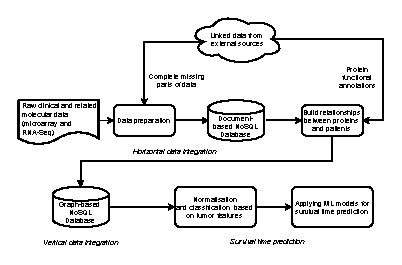
\includegraphics{Fig3.eps}
  \caption{
    \csentence{
         Workflow of data integration of independent datasets, performed
within our framework. 
    }
    In data preparation phase we transform and store raw data with different formats in a document database which is considered as horizontal data integration. After that we generate the relations between data based on the raw dataset for patients, molecular data and we store them in a graph based database thus we developed the internal network. After that for every mutation we search related information from external knowledge sources and build the new general relations network which is considered as vertical data integration. We store these enriched relations in the graph based database together with the internal relationships.
  }
  \label{figure_3}
\end{figure}



\begin{figure}[h!]
  \centering
  \includegraphics{Fig4.eps}
  \caption{
    \csentence{
         TICF complex feature.
    }
     TICF consists of three concatenated
parameters: tumor stage, tumor size and age at diagnosis. The columns
virtually group the patients by TICF, with regard to the first number
{}-- the tumor stage. The rows (split by dotted lines) sort patients
according to the values of the TICF referring to the tumor size and age
at diagnosis {}-- from left to right following the growth of numerical
axis. 
  }
  \label{figure_4}
\end{figure}



\begin{figure}[h!]
  \centering
  \includegraphics{Fig5.eps}
  \caption{
    \csentence{
         Example of semantically related patients based on internal and
linked network.
    }
     The studied patient is shown as a larger circle in the
middle. The vertical lines split the schema into 5 classes, as
determined by the k-neighbor classification of the TICF feature. Black
arrows show patients related to the studied patient based on the
internal relationships. Grey arrows distinguish patients related to the
studied patient based on linked data (from EDKS).
  }
  \label{figure_5}
\end{figure}


\begin{figure}[h!]
  \centering
  \includegraphics{Fig6.eps}
  \caption{
    \csentence{
         Success rates of machine learning models for survival time
prediction as mapping of predicted-to-measured values of survival time
prediction (by TICF).
    }
     Numbers correspond to months of survival time
prediction. A dotted line symbolizes an ideal case of the ratio
predicted to measured TICF for survival time prediction.
  }
  \label{figure_6}
\end{figure}



\begin{figure}[h!]
  \centering
  \includegraphics{Fig7.eps}
  \caption{
    \csentence{
          Cross-validation of the applied machine learning models for
survival time prediction.
    }
     Performance of three models (SVR-Linear,
SVR-RBF and DTR) is compared. The fourth model, SVR-Poly has shown
biased results (Fig.~\ref{figure_5}). Cross-validation is based on 5 subgroups
defined by the TICF feature, obtained after using k-fold algorithm. On
the vertical axis the mean values with standard deviations of success
rates and error rates of the matchings of TICF feature are given.
  }
  \label{figure_7}
\end{figure}

%%%%%%%%%%%%%%%%%%%%%%%%%%%%%%%%%%%
%%                               %%
%% Tables                        %%
%%                               %%
%%%%%%%%%%%%%%%%%%%%%%%%%%%%%%%%%%%

\begin{table}[h!]
\caption{Aggregated results of cross-validation.}
   \begin{tabular}{ccccccccc}
{\textbf{ML Model}} &  \multicolumn{2}{c}{{\textbf{Train R2}}} & \multicolumn{2}{c}{{\textbf{Explained Variance}}} & \multicolumn{2}{c}{\textbf{Negative Mean}} & \multicolumn{2}{c}{\textbf{Negative Median}}\\ & & & & & \multicolumn{2}{c}{\textbf{Absolute Error}} & \multicolumn{2}{c}{\textbf{Absolute Error}} \\
\midrule
{} & \textbf{Mean} & \textbf{StD} & \textbf{Mean} & \textbf{StD} & \textbf{Mean} & \textbf{StD} & \textbf{Mean} & \textbf{StD}\\
SVR-RBF & 0.318 & 0.038 & 0.341 & 0.032 & $-$45.742 & 5.224 & $-$34.455 & 5.594\\
SVR-LINEAR & 0.983 & 0.007 & 0.986 & 0.006 & $-$7.288 & 1.935 & $-$6.109 & 1.509\\
DTR & 0.996 & 0.000 & 0.996 & 0.427 & $-$5.624 & 0.427 & $-$4.636 & 0.467\\
SVR-POLY & 0.884 & 0.007 & 0.887 & 0.009 & $-$20.354 & 3.290 & $-$15.581 & 5.382\\
\bottomrule
\end{tabular}
\end{table}

\begin{table}[h!]
\caption{Execution time of the applied ML models per iteration. in terms of time of training, predict and total time which are sum of the train plus predict time.}  \label{tab2}
\centering
%% \tablesize{} %% You can specify the fontsize here, e.g.,  \tablesize{\footnotesize}. If commented out \small will be used.
\begin{tabular}{cccc}
\toprule
\textbf{ML Model} & \textbf{Train (s)} & \textbf{Predict (s)} & \textbf{Total (s)} \\
\midrule
SVR-RBF & 0.070589066 & 0.001976013 & 0.072565079 \\
SVR-LINEAR & 0.050335884 & 0.000173092 & 0.050508976 \\
DTR & 0.028145075 & 0.000221968 & 0.028367043 \\
SVR-POLY & 0.479592085 & 0.001157999 & 0.480750084 \\
\bottomrule
\end{tabular}
\end{table}


%% Use of \listoftables is discouraged.
%%
%\section*{Tables}
%\begin{table}[h!]
%\caption{Sample table title. This is where the description of the table should go.}
%      \begin{tabular}{cccc}
%        \hline
%           & B1  &B2   & B3\\ \hline
%        A1 & 0.1 & 0.2 & 0.3\\
%        A2 & ... & ..  & .\\
%        A3 & ..  & .   & .\\ \hline
%      \end{tabular}
%\end{table}

%%%%%%%%%%%%%%%%%%%%%%%%%%%%%%%%%%%
%%                               %%
%% Additional Files              %%
%%                               %%
%%%%%%%%%%%%%%%%%%%%%%%%%%%%%%%%%%%

%\section*{Additional Files}
%  \subsection*{Additional file 1 --- Sample additional file title}
%    Additional file descriptions text (including details of how to
%    view the file, if it is in a non-standard format or the file extension).  This might
%    refer to a multi-page table or a figure.
%
%  \subsection*{Additional file 2 --- Sample additional file title}
%    Additional file descriptions text.
%

\end{backmatter}
\end{document}

